\chapter{Detalles de Implementación y Experimentos}\label{chapter:implementation}

\section{Aplicación para la captura de señales}
	Para capturar las señales se utilizó una aplicación implementada en \emph{Flutter} 2.10.15, con \emph{dart} 2.16.2.
	Se utlizaron las bibliotecas \emph{sensors\textunderscore plus} y \emph{geolocator} para obtener acceso a las lecturas del \textbf
	{acelerómetro}, \textbf{giroscopio} y \textbf{GPS}. Para comenzar a realizar una captura se aprieta el botón de \emph{Start recorder}
	y a partir de ese momento la aplicación comienza a reflejar los valores que se obtienen de los sensores en la interfaz de usuario.\\
	\indent La aplicación muestra en tiempo real las lecturas de los distintos sensores, así como la velocidad en kilómetros por hora (km/h) y la
	duración de la captura que se está realizando en el momento (ver figura \ref{fig:6}).\\
	\indent Cuando se desea detener la grabación se presiona el botón \emph{Stop recorder}. Luego si se quiere exportar dicha grabación se puede
	hacer presionando el botón de \emph{Save record as} e introduciendo el nombre con el que se desea salvar dichar grabación (ver figura
	\ref{fig:7}). De esta forma se puede acceder a todas las grabaciones para posteriormente utilizarlas en el modelo de aprendizaje de máquinas.\\
	\indent Con el botón \emph{Mark anomaly} se pueden realizar marcas, de esta forma se salvan las coordenadas de latitud-longitud en un
	archivo de marcas. La aplicación tiene además un mapa donde se pueden visualizar datos de latitud-longitud previamente guardados.
	Estos se pueden cargar en la pestaña del mapa de la aplicación para poder visualizar dichas marcas en el mapa (ver figura \ref{fig:8}).
	De esta forma se pueden marcar los baches y verlos en un mapa.\\
	
	\begin{figure}[htb]
		\centering
		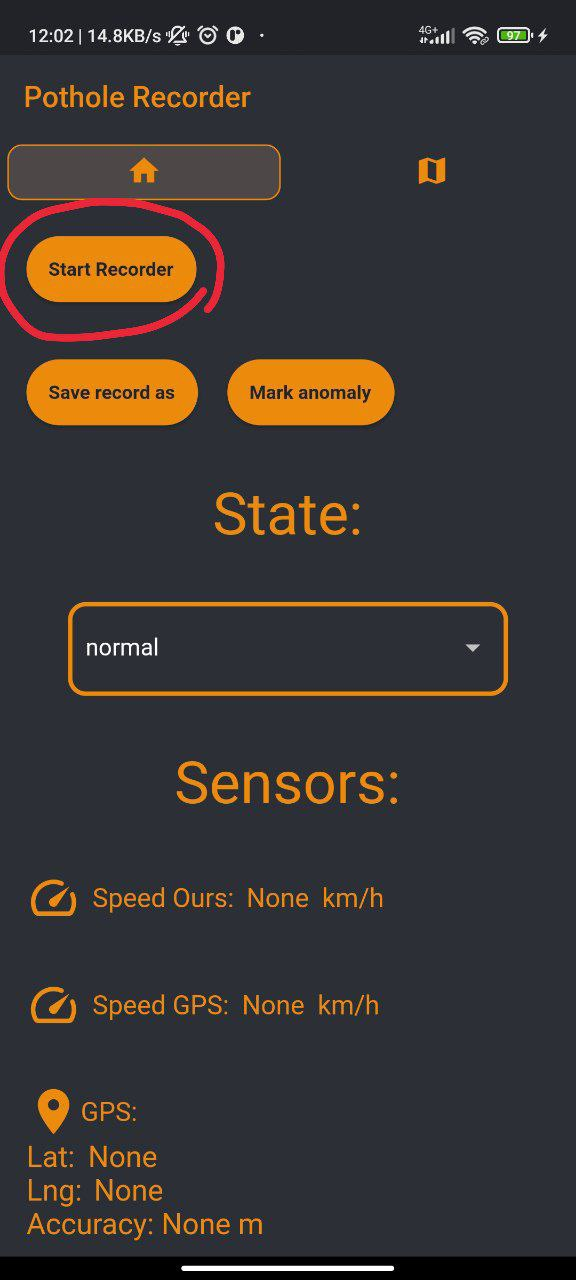
\includegraphics[scale = 0.2]{Graphics/apk_start_recording.jpg}
		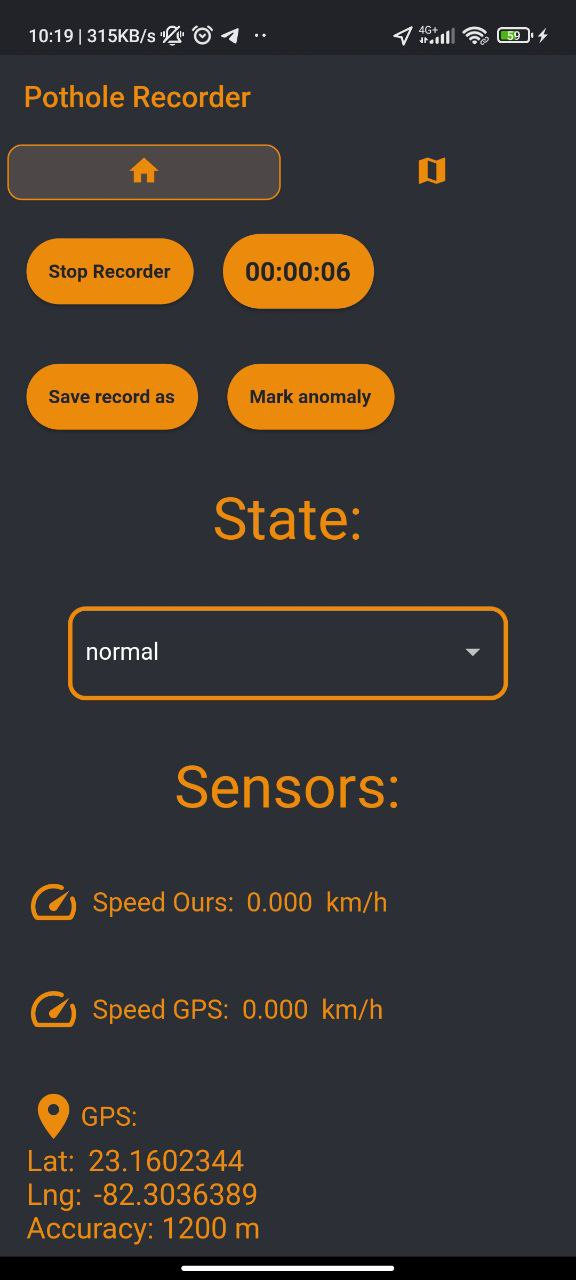
\includegraphics[scale = 0.2]{Graphics/apk_recording_ui.jpg}
		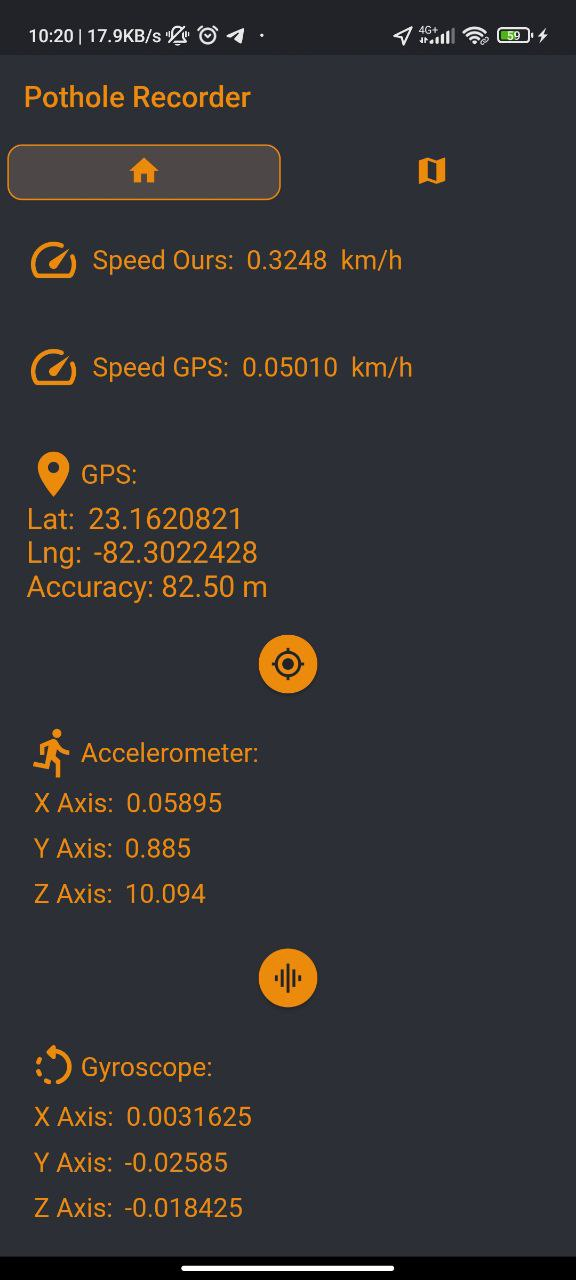
\includegraphics[scale = 0.2]{Graphics/apk_recording_sensors.jpg}
		\caption{Comenzar a grabar y lecturas reflejadas en la aplicación}
		\label{fig:6}
	\end{figure}
	\newpage

	\indent Es necesario dar permisos de escritura para salvar en el dispositivo móvil los archivos que se obtienen como resultado del 
	muestreo de los sensores, los archivos exportados y el archivo donde se almacenan las marcas que se realizan manualmente. Estos archivos
	se guardan en un directorio nombrado \textbf{Baches} en la raíz del almacenamiento interno del dispositivo móvil.\\
	\indent En esta carpeta hay otras 3 carpetas:

	\begin{itemize}
		\item \textbf{mark\textunderscore labels}: Donde se guardan las marcas.
		\item \textbf{sensors}: Donde se guarda el archivo temporal en el que se van guardando los datos que va recopilando la aplicación
			mientras está grabando.
		\item \textbf{exported} donde se guardan los archivos exportados.
	\end{itemize}

	Además, es necesario dar permisos de ubicación a la aplicación para que pueda acceder a los datos del \textbf{GPS}, latitud y longitud,
	en tiempo real.

	\begin{figure}[htb]
		\centering
		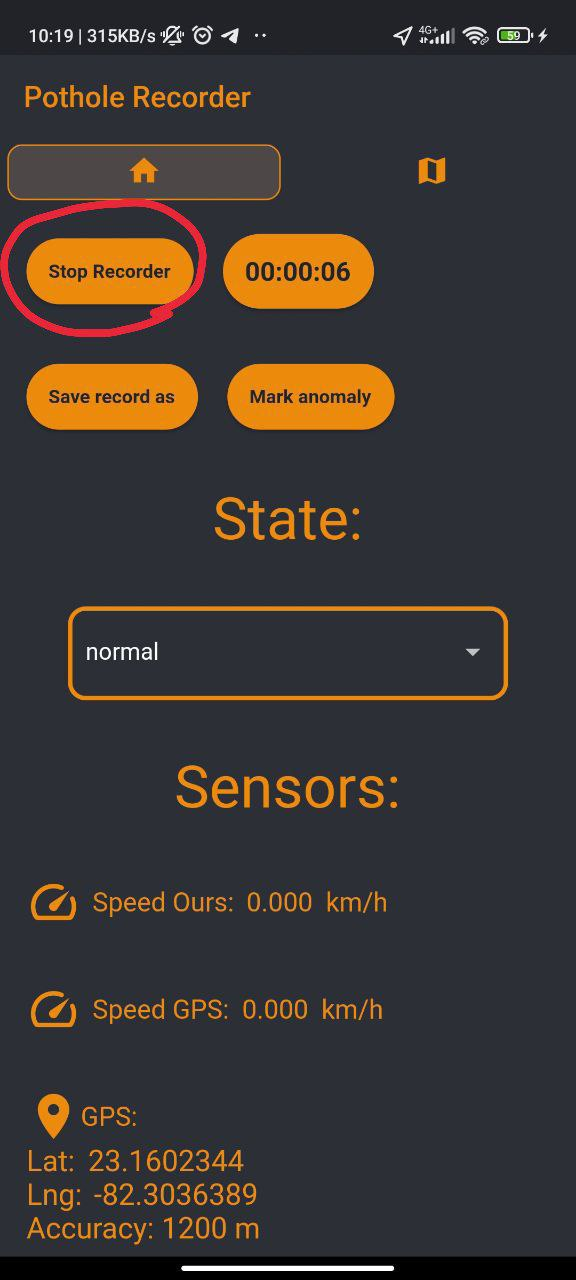
\includegraphics[scale = 0.175]{Graphics/apk_stop_recording.jpg}
		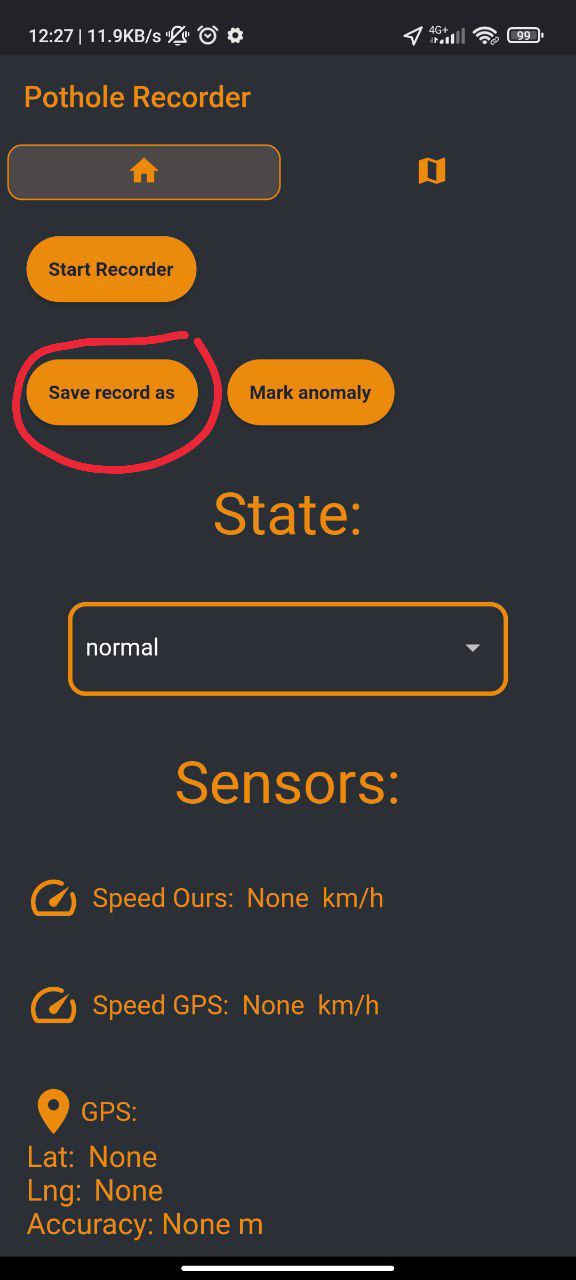
\includegraphics[scale = 0.175]{Graphics/apk_save_recording_1.jpg}
		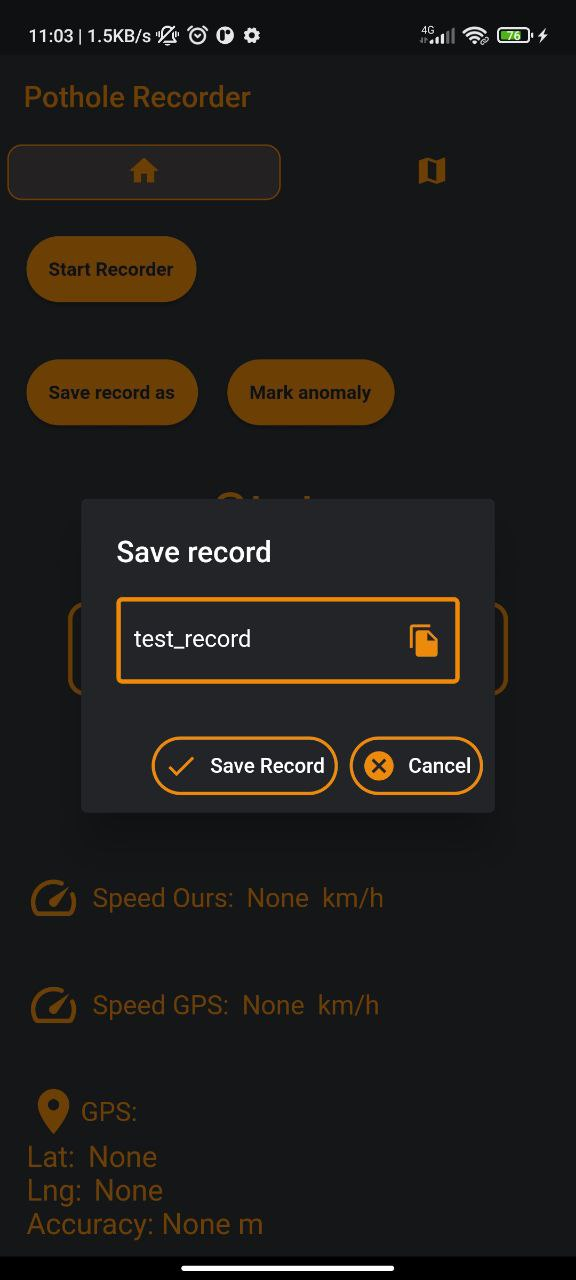
\includegraphics[scale = 0.175]{Graphics/apk_save_recording_2.jpg}
		\caption{Detener grabación y exportar}
		\label{fig:7}
	\end{figure}

	\begin{figure}[htb]
		\centering
		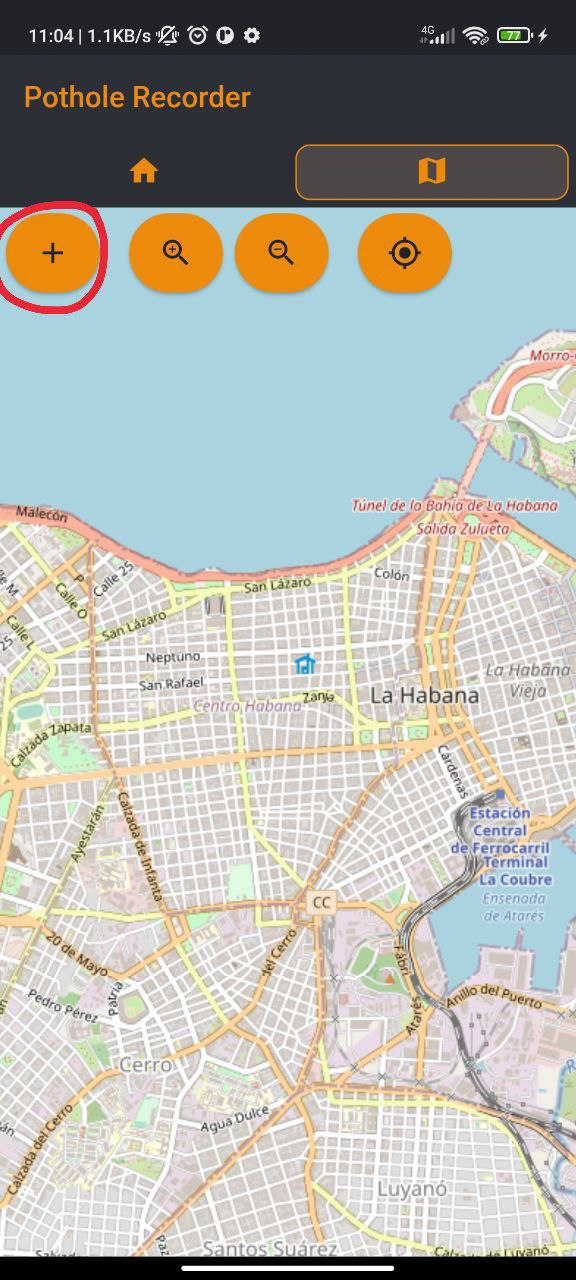
\includegraphics[scale = 0.175]{Graphics/load_marks_to_map_1.jpg}
		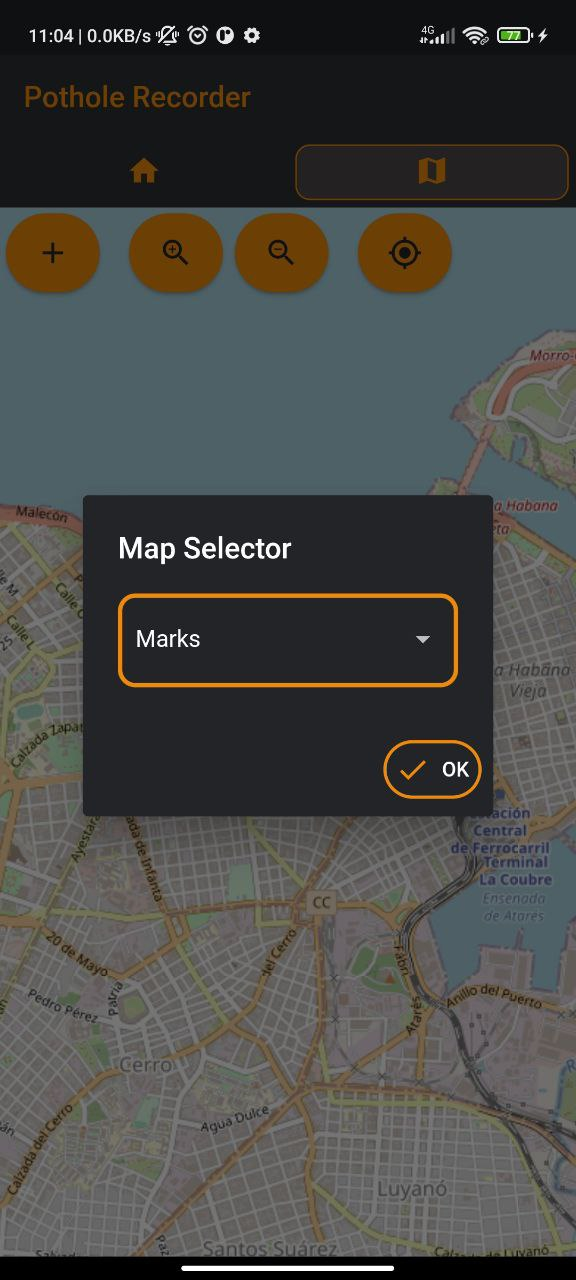
\includegraphics[scale = 0.175]{Graphics/load_marks_to_map_2.jpg}
		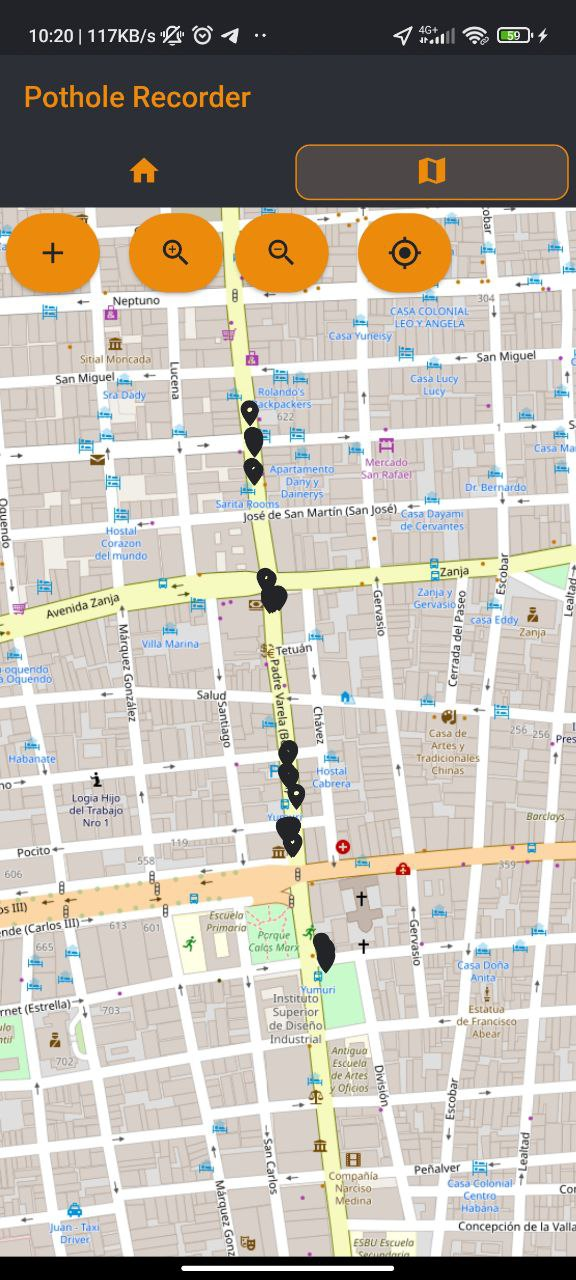
\includegraphics[scale = 0.175]{Graphics/map_marks_apk.jpg}
		\caption{Cargar marcas en el mapa de la aplicación}
		\label{fig:8}
	\end{figure}
	\newpage

	Los datos se guardan en archivos .\textbf{JSON}. Las marcas guardan \textbf{latitud}, \textbf{longitud}, \textbf{precisión} y una 
	etiqueta para indicar que en esa ubicación hay un bache. Por otro lado, las lecturas guardan \textbf{aceleración} en los 3 ejes, 
	\textbf{velocidad de giro} en los 3 ejes, \textbf{latitud}, \textbf{longitud}, \textbf{precisión}, \textbf{velocidad}, \textbf{estado}
	y \textbf{frecuencia de muestreo}. Estos datos se almacenan en el archivo temporal y en los datos una vez exportados. En este último, también 
	se guarda la duración en milisegundos, del recorrido realizado.

	La aplicación cuenta además, con una funcionalidad que permite etiquetar ciertas capturas con frases como \textbf{girar izquierda},
	\textbf{girar derecha}, \textbf{frenar} y \textbf{normal}. Con estas estiquetas, se puede registrar cuando el vehículo dobla en alguna
	esquina o cuando frena, mientras se captura la señal. Esto puede ser útil para descartar anomalías asociadas a estos eventos o
	para mostrar y analizar el comportamiento de las señales de los sensores mientras el vehículo se encuentra en alguno de estos estados
	(ver figura \ref{fig:9}).

	\begin{figure}[htb]
		\centering
		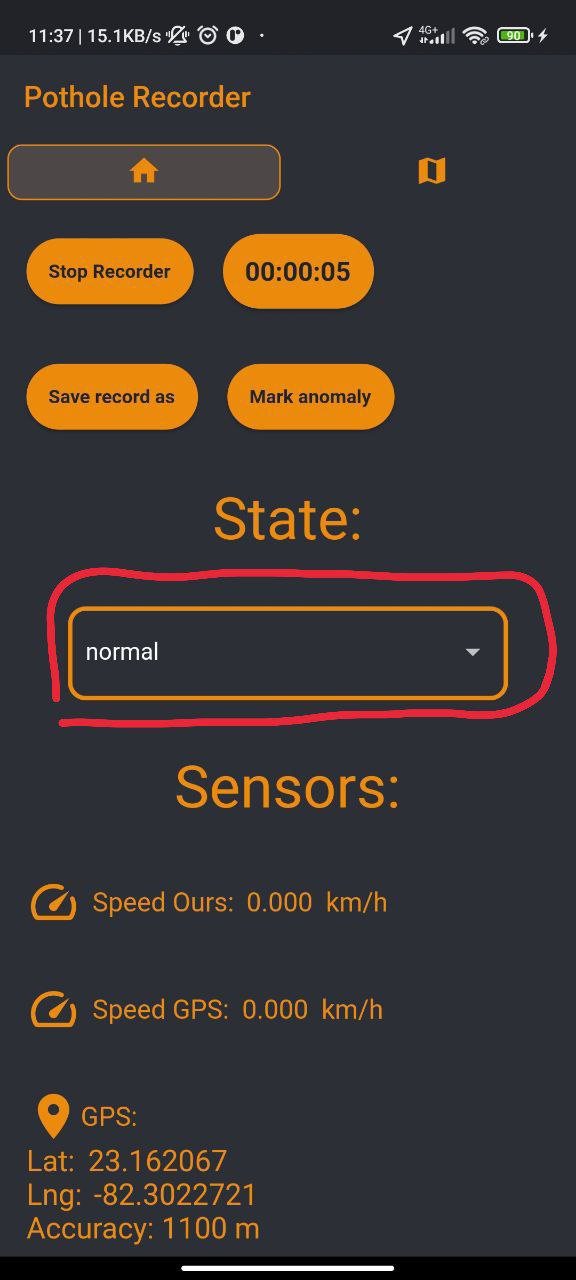
\includegraphics[scale = 0.2]{Graphics/apk_change_state_1.jpg}
		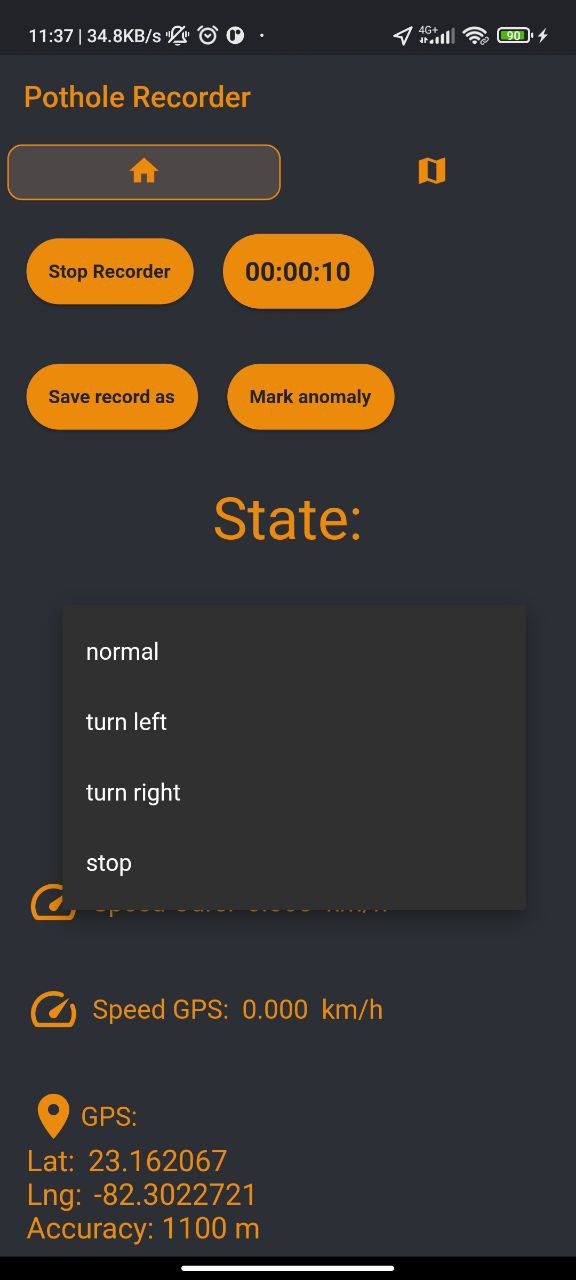
\includegraphics[scale = 0.2]{Graphics/apk_change_state_2.jpg}
		\caption{Cargar marcas en el mapa de la aplicación}
		\label{fig:9}
	\end{figure}

	\subsection{\emph{Hardware} y \emph{software} en el que se probó la aplicación}
		La aplicación se probó en dos dispositivos móviles. Un \textbf{Xiaomi Mi A2} y un \textbf{Xiaomi Redmi 10} con \textbf{Android 9} y
		\textbf{11} respectivamente. Ambos dispositivos tienen \textbf{acelerómetro}, \textbf{giroscopio} y \textbf{GPS}. El dispositivo que 
		se escogió para capturar las señales y realizar las marcas de los baches fue el \textbf{Xiaomi Redmi 10}, debido a que este tenía mejor
		precisión en las lecturas del \textbf{GPS}, las cuales se mantuvieron en un rango de 1.3 a 9 metros. En el \textbf{Xiaomi Mi A2}, las 
		lecturas del \textbf{GPS} se mantuvieron generalmente por encima de 50 metros, rara vez por debajo de esa cifra.

	\subsection{Metodología para la captura de señales}
		Primero que todo, para capturar las señales, escogimos varias rutas de La Habana de longitud moderada. Luego nos montamos en un vehículo
		y colocamos el dispositivo en el asiento de tal forma que su eje Y coindiera con el eje Y del vehículo y su pantalla estuviera hacia arriba.
		Apenas el vehículo comenzó a moverse pusimos la aplicación a grabar. Durante el viaje, dado que no se contaba con un objeto capaz de fijar el
		dispositivo móvil en la posición deseada, se tuvo que sostener lo mejor posible con las manos para que mantuviera la orientación. \\
		\indent Cuando el vehículo se iba a detener por alguna razón y se estaba al tanto, se cambiaba al estado de \textbf{frenar} un poco antes, para
		registrar tal evento en los datos. Lo mismo se hizo cuando el vehículo iba a doblar una esquina. Una vez terminaba el evento, se cambiaba otra
		vez a estado \textbf{normal}. Cuando el vehículo llegaba al final de la ruta planeada, se detenía el proceso de grabación y se exportaban los
		datos de dicho recorrido a un archivo .\textbf{JSON} aparte con un nombre que indentificara la ruta.

	\subsection{Metodología para marcar los baches}
		Para marcar los baches, se recorrió la misma ruta que se había seleccionado para capturar los datos, y se fueron marcando los baches. Antes 
		de realizar las marcas, se esperó un tiempo a que la precisión del \textbf{GPS} se estabilizara en un rango aceptable, preferiblemente por debajo 
		de los 5 metros. Las marcas se realizaron desde la acera debido al tráfico, y en la medida de lo posible un poco más cerca del bache en la calle.
		Por cada bache, se realizaron varias marcas con distinta precisión y desde distintas ubicaciones relativamente cercanas a la ubicación real del
		bache, con el objetivo de minimizar el efecto del error inherente del \textbf{GPS}.

	\subsection{Error en las lecturas y las marcas}
		En las lecturas durante los recorridos existe cierto error. Esto se debe a que no se pudo fijar el dispositivo en la posición óptima y se tuvo que
		sostener con las manos, lo que sin duda alguna influye negativamente en los datos obtenidos. También, en estas lecturas y en las marcas, hay un
		error inherente del propio \textbf{GPS}. En las marcas además, hay un error extra debido a que estas se realizaron de la acera.

\section{Aplicación para los modelos de aprendizaje de máquinas}
